\documentclass[25pt, a0paper, portrait]{tikzposter}
\usetheme{Rays}
\usecolorstyle{Default}
\usepackage[utf8]{inputenc}
\usepackage[T1]{fontenc}
\usepackage[english]{babel}
\usepackage{amsmath,amssymb}
\usepackage{tikz}
\usetikzlibrary{shapes.geometric, arrows, calc, positioning}

\title{Makeitalive: Landscape picture animation}
\author{Mathurin Petit, Arthur Fournier}
\institute{CSC\_52002 - Generative AI Project}

\begin{document}
\maketitle

\begin{columns}
    \column{0.5}
    \block{1. Project Overview}{
        The \textbf{Makeitalive} project explores the transformation of a static landscape photograph into a realistic animation. 
        We preserve the original texture while injecting coherent movement.
        
        \vspace{1em}
        \textbf{Challenges met:}
        \begin{itemize}
            \item Automatic animation.
            \item HD temporal coherence.
            \item Realism of natural textures.
        \end{itemize}
    }
    
    \block{2. The Motion Flow Concept}{
        The approach is based on estimating an \textit{Optical Flow} field:
        \begin{itemize}
            \item Prediction of $(dx, dy)$ vectors per pixel.
            \item \textbf{Backward Mapping} for rendering:
            \[ I_{anim}(x, y, t) = I_{orig}(x - \alpha_t dx, y - \alpha_t dy) \]
        \end{itemize}
    }

    \block{3. Model Architectures}{
    \begin{minipage}[t]{0.45\linewidth}
        \centering
        \textbf{Motion Flow U-Net}
        
        \vspace{0.5em}
        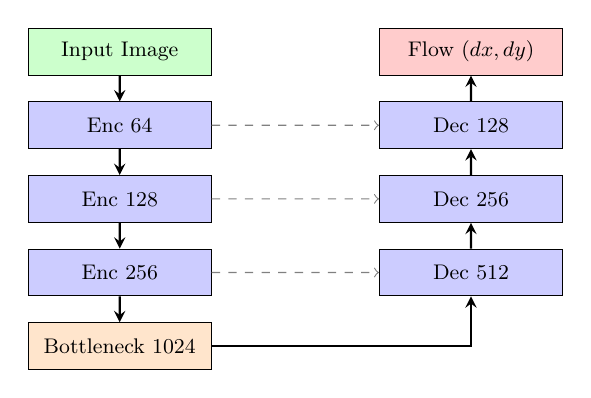
\begin{tikzpicture}[node distance=1.1cm, scale=0.85, transform shape]
            \tikzstyle{layer} = [rectangle, draw, fill=blue!20, text width=2.5cm,
                                 text centered, minimum height=0.7cm, font=\small]
            \tikzstyle{flow} = [->, >=stealth, thick]

            \node (in)   [layer, fill=green!20]          {Input Image};
            \node (enc1) [layer, below of=in]            {Enc 64};
            \node (enc2) [layer, below of=enc1]          {Enc 128};
            \node (enc3) [layer, below of=enc2]          {Enc 256};
            \node (btl)  [layer, below of=enc3, fill=orange!20] {Bottleneck 1024};
            \node (dec3) [layer, right=2.5cm of enc3]    {Dec 512};
            \node (dec2) [layer, right=2.5cm of enc2]    {Dec 256};
            \node (dec1) [layer, right=2.5cm of enc1]    {Dec 128};
            \node (out)  [layer, right=2.5cm of in, fill=red!20] {Flow $(dx,dy)$};

            \draw [flow] (in) -- (enc1);
            \draw [flow] (enc1) -- (enc2);
            \draw [flow] (enc2) -- (enc3);
            \draw [flow] (enc3) -- (btl);
            \draw [flow] (btl) -| (dec3);
            \draw [flow] (dec3) -- (dec2);
            \draw [flow] (dec2) -- (dec1);
            \draw [flow] (dec1) -- (out);
            \draw [dashed, ->, gray] (enc1) -- (dec1);
            \draw [dashed, ->, gray] (enc2) -- (dec2);
            \draw [dashed, ->, gray] (enc3) -- (dec3);
        \end{tikzpicture}
    \end{minipage}
    \hfill
    \begin{minipage}[t]{0.45\linewidth}
        \centering
        \textbf{SVD (fine-tuned)}
        
        \vspace{0.5em}
        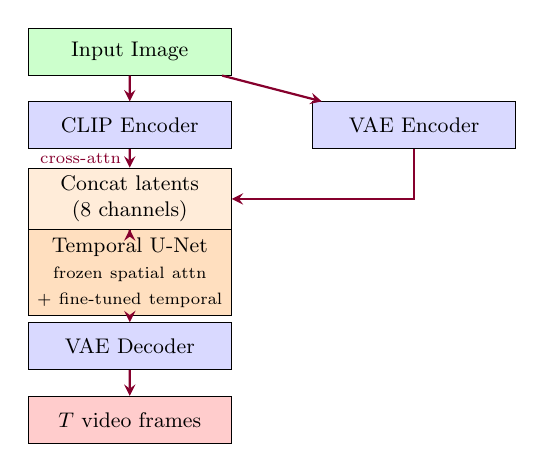
\begin{tikzpicture}[node distance=1.1cm, scale=0.85, transform shape]
            \tikzstyle{svd} = [rectangle, draw, fill=purple!20, text width=2.8cm,
                               text centered, minimum height=0.7cm, font=\small]
            \tikzstyle{sf} = [->, >=stealth, thick, purple!70!black]

            \node (img)  [svd, fill=green!20]             {Input Image};
            \node (clip) [svd, fill=blue!15, below of=img] {CLIP Encoder};
            \node (vae)  [svd, fill=blue!15, right=1.2cm of clip] {VAE Encoder};
            \node (cat)  [svd, fill=orange!15, below of=clip] {Concat latents\\(8 channels)};
            \node (unet) [svd, fill=orange!25, below of=cat, text width=2.8cm]
                         {Temporal U-Net\\{\scriptsize frozen spatial attn}\\{\scriptsize + fine-tuned temporal}};
            \node (dec)  [svd, fill=blue!15, below of=unet] {VAE Decoder};
            \node (vid)  [svd, fill=red!20,  below of=dec]  {$T$ video frames};

            \draw [sf] (img)  -- (clip);
            \draw [sf] (img)  -- (vae);
            \draw [sf] (clip) -- node[left, font=\scriptsize]{cross-attn} (cat);
            \draw [sf] (vae)  |- (cat);
            \draw [sf] (cat)  -- (unet);
            \draw [sf] (unet) -- (dec);
            \draw [sf] (dec)  -- (vid);
        \end{tikzpicture}
    \end{minipage}

    \vspace{1em}
    \begin{center}
    \begin{tabular}{|l|c|c|}
        \hline
        & \textbf{Motion Flow} & \textbf{SVD} \\
        \hline
        Parameters  & $<$100MB   & 1.5B \\
        Output      & Flow $(dx,dy)$ & Video frames \\
        Training    & MSE on flow & EDM diffusion loss \\
        Inference   & Real-time  & $\sim$25s / clip \\
        \hline
    \end{tabular}
    \end{center}
}

    \column{0.5}
    \block{4. Stable Video Diffusion (SVD) Approach}{
    \textbf{Pipeline overview:}
    \begin{itemize}
        \item YouTube drone videos → frame extraction with \texttt{frame\_gap=12} (captures $\sim$7s of real motion per clip)
        \item Motion filtering: $3.0 < \text{score} < 40.0$ (rejects static scenes and hard cuts)
        \item Fine-tuning via \textbf{SVD\_Xtend}: full UNet training, $lr=10^{-5}$, 5000 steps
    \end{itemize}

    \vspace{0.5em}
    \textbf{Key design choices:}
    \begin{itemize}
        \item \texttt{noise\_aug\_strength=0.02}: adds noise to conditioning frame, closes train/inference gap
        \item CFG dropout: enables guidance scale control at inference
        \item Post-processing: raw 7fps output slowed to 2fps $\rightarrow$ interpolated to 24fps via \texttt{ffmpeg minterpolate}
    \end{itemize}

    \vspace{0.5em}
    \textbf{Loss convergence (SVD\_Xtend, 2374 clips):}
    \begin{center}
    \begin{tabular}{|c|c|}
        \hline
        \textbf{Steps} & \textbf{Step Loss} \\
        \hline
        500   & $\sim$0.60 \\
        1000  & $\sim$0.45 \\
        3000  & $\sim$0.16 \\
        5000  & $\sim$0.20 \\
        \hline
    \end{tabular}
    \end{center}
}

    \block{5. Comparison of Techniques}{
        \begin{center}
        \begin{tabular}{|l|c|c|}
            \hline
            \textbf{Criterion} & \textbf{Motion Flow} & \textbf{SVD + LoRA} \\
            \hline
            Fidelity & Maximum & High \\
            Speed & Instant & Several seconds \\
            Weight & Light & Heavy \\
            Resources & CPU/GPU & High-End GPU \\
            \hline
        \end{tabular}
        \end{center}
    }

    \block{6. Result Evaluation}{
    \textbf{Qualitative comparison} (INPUT $\rightarrow$ GENERATED $\rightarrow$ GROUND TRUTH):
    \begin{itemize}
        \item SVD\_Xtend produces coherent drone-style camera motion on landscape images
        \item Motion fidelity improves significantly vs.\ naive LoRA ($\Delta \text{loss} \approx -0.30$)
        \item Remaining limitations: interpolation artifacts on high-frequency textures (dense foliage), and motion amplitude constrained by \texttt{motion\_bucket\_id}
    \end{itemize}

    \vspace{0.5em}
    \textbf{Ablation — impact of dataset quality:}
    \begin{center}
    \begin{tabular}{|l|c|c|}
        \hline
        \textbf{Setup} & \textbf{Final Loss} & \textbf{Motion quality} \\
        \hline
        LoRA, static clips        & 0.46 & None \\
        LoRA, motion-filtered     & 0.51 & Minimal \\
        SVD\_Xtend, motion-filtered & 0.16 & Cinematic \\
        \hline
    \end{tabular}
    \end{center}
}

    \block{7. Conclusion}{
        The hybridization of the two delivers the best of both worlds: structural speed and generative textual richness.
    }
\end{columns}

\end{document}
